\documentclass[11pt,letterpaper]{article}
\usepackage[T1]{fontenc}
\usepackage[utf8]{inputenc}
\usepackage[spanish,english,es-tabla,es-noquoting,es-nodecimaldot]{babel}
\usepackage{newtxtext,newtxmath}
\renewcommand{\ttdefault}{lmtt}
\usepackage{amsmath}
\usepackage[locale=US]{siunitx}
\sisetup{group-separator={\,},group-minimum-digits=4,separate-uncertainty=true,output-decimal-marker={.}}
\usepackage{booktabs,graphicx,float,array,tabularx,longtable}
\usepackage[labelsep=period,font=small,labelfont=bf]{caption}
\usepackage[margin=2.4cm]{geometry}
\usepackage{xcolor}
\definecolor{navy}{HTML}{1F3B63}
\usepackage{titlesec}
\titleformat{\section}{\normalfont\Large\bfseries}{\thesection.}{0.6em}{}
\titleformat{\subsection}{\normalfont\large\bfseries}{\thesubsection}{0.6em}{}
\titlespacing*{\section}{0pt}{14pt}{6pt}
\titlespacing*{\subsection}{0pt}{10pt}{4pt}
\usepackage{enumitem}
\setlist{itemsep=1pt,topsep=3pt}
\setlist[itemize]{label=$\bullet$}
\usepackage{listings}
\lstset{language=Python,basicstyle=\ttfamily\footnotesize,breaklines=true,frame=single,rulecolor=\color{black!40},showstringspaces=false,columns=fullflexible,keepspaces=true,extendedchars=true,literate={á}{{\'a}}1 {é}{{\'e}}1 {í}{{\'i}}1 {ó}{{\'o}}1 {ú}{{\'u}}1 {ñ}{{\~n}}1}
\usepackage{fancyhdr}
\pagestyle{fancy}\fancyhf{}
\fancyhead[L]{\small Análisis espectral de Fourier para alertas sísmicas}
\fancyhead[R]{\small\thepage}
\renewcommand{\headrulewidth}{0.4pt}
\setlength{\headheight}{14pt}
\usepackage{csquotes}
\usepackage[style=apa,backend=biber]{biblatex}
\addbibresource{refs.bib}
\usepackage{hyperref}
\hypersetup{colorlinks,allcolors=black,urlcolor=navy}
\setlength{\parindent}{0pt}
\setlength{\parskip}{5pt}
\setcounter{tocdepth}{1}
\newcommand{\fuente}{Fuente: elaboración propia.}
\newtheorem{prop}{Proposición}

\begin{document}
\selectlanguage{spanish}

% ================= PORTADA =================
\begin{titlepage}
\centering
{\large\bfseries Instituto Tecnológico y de Estudios Superiores de Monterrey\par}
\vspace{2pt}
{\large Campus Monterrey\par}
\vspace{1.2cm}
{\large Análisis de Métodos Matemáticos para la Física\par}
\vfill
{\color{navy}\rule{\textwidth}{1.2pt}}\par\vspace{0.6cm}
{\large\scshape Reporte técnico final\par}\vspace{0.3cm}
{\fontsize{24}{30}\selectfont\bfseries Análisis espectral de Fourier para alertas\\[4pt] de señales sísmicas inclusivas\par}
\vspace{0.5cm}
{\large Separación de la onda sísmica y del ruido ambiental para el Earthquake Hazards Program del USGS. Del modelo con series de Fourier a la transformada por ventanas en 20 sismos reales de México\par}
\vspace{0.6cm}
{\color{navy}\rule{\textwidth}{1.2pt}}\par
\vfill
{\large\bfseries Equipo\par}
\vspace{6pt}
\begin{tabular}{ll}
Mateo Rodolfo Flores Torres & A01783438\\
Víctor Manuel Sánchez Chávez & A01287522\\
Sofía Martínez Alanis & A01724528\\
\end{tabular}
\par\vspace{0.8cm}
{\large Profesor: Dr. Luis Miguel Méndez Díaz\par}
\vspace{4pt}
{\normalsize Prototipo y código: \url{https://sismo-o-ruido.vercel.app} · \url{https://github.com/Mmateo101/video-fismat}\par}
\vspace{1.0cm}
{\large Monterrey, Nuevo León, noviembre de 2026\par}
\end{titlepage}

% ================= RESUMEN =================
\section*{Resumen}
\addcontentsline{toc}{section}{Resumen}
El Earthquake Hazards Program del USGS necesita separar la onda de un sismo del ruido ambiental que registran sus sensores, porque de esa separación depende que una alerta temprana sea oportuna y confiable. Este trabajo modela la señal registrada como la superposición de un campo de onda sísmico y un campo de ruido, y la analiza con herramientas de física matemática. En una primera etapa se estudian dos registros simplificados del USGS con la serie de Fourier discreta en su forma compleja. La ortogonalidad de las raíces de la unidad da los coeficientes, y el teorema de Parseval muestra que un armónico de \SI{4.2}{s} concentra el \SI{94.8}{\percent} de la varianza. Una regresión trigonométrica por mínimos cuadrados da amplitudes de $0.365 \pm 0.021$ y $0.062 \pm 0.002$. De la ecuación de onda se deduce la energía media, que da un cociente de $35 \pm 5$, y la relación de dispersión da una longitud de onda de unos \SI{18}{km}. El periodo dominante coincide con el de los microsismos oceánicos, así que la frecuencia sola no basta. Por eso, en una segunda etapa el modelo se lleva al límite de la transformada integral de Fourier y se aplica por ventanas a 20 sismos reales de México registrados en Ciudad Universitaria. El ruido se estima antes de la onda P y se resta con una ganancia que se deduce como estimador de mínimo error cuadrático. La relación señal-ruido mejora en los 20 sismos, en promedio \SI{10.5}{dB}. Con ruido real tan fuerte como el sismo, la correlación con la onda verdadera sube de 0.71 a 0.86.

\textbf{Palabras clave:} serie de Fourier compleja, teorema de Parseval, transformada de Fourier, teorema de convolución, potenciales de Helmholtz, filtro de Wiener, ruido sísmico.

\begin{otherlanguage}{english}
\section*{Abstract}
\addcontentsline{toc}{section}{Abstract}
The USGS Earthquake Hazards Program must separate the earthquake wave from the ambient noise its sensors record, because timely and reliable early warnings depend on it. This work models the recorded signal as the superposition of a seismic wave field and a noise field and analyzes it with tools of mathematical physics. First, two simplified USGS records are studied with the complex discrete Fourier series. Orthogonality of the roots of unity gives the coefficients, and Parseval's theorem shows that a \SI{4.2}{s} harmonic holds \SI{94.8}{\percent} of the variance. A least-squares trigonometric regression gives amplitudes of $0.365 \pm 0.021$ and $0.062 \pm 0.002$. The mean energy derived from the wave equation gives a ratio of $35 \pm 5$, and the dispersion relation gives a wavelength of about \SI{18}{km}. The dominant period matches oceanic microseisms, so frequency alone is not enough. The model is therefore taken to the Fourier integral transform and applied in windows to 20 real Mexican earthquakes recorded at Ciudad Universitaria. Noise is estimated before the P wave and removed with a gain derived as a minimum mean-square-error estimator. The signal-to-noise ratio improves for all 20 earthquakes, by \SI{10.5}{dB} on average. With real noise as strong as the earthquake, the correlation with the true wave rises from 0.71 to 0.86.

\textbf{Keywords:} complex Fourier series, Parseval's theorem, Fourier transform, convolution theorem, Helmholtz potentials, Wiener filter, seismic noise.
\end{otherlanguage}

\clearpage
\tableofcontents
\clearpage

% ================= 1 INTRODUCCIÓN =================
\section{Introducción}
Los sismos están entre los riesgos naturales más letales. Varios terremotos del último siglo causaron más de \num{150000} muertes cada uno \parencite{statista2025}. Un sistema de alerta temprana detecta las primeras ondas de un sismo y avisa antes de que lleguen las sacudidas fuertes \parencite{allen2019}. México opera el SASMEX desde 1991 \parencite{espinosa1995} y Estados Unidos opera ShakeAlert a través del Earthquake Hazards Program (EHP) del USGS \parencite{usgs_ehp,usgs_anss}.

El EHP planteó a nuestro equipo una pregunta concreta \parencite{expediente}. Un sensor registra a la vez la onda del sismo y el ruido ambiental. ¿Cómo separarlos con herramientas matemáticas para que la alerta no se dispare con el ruido ni llegue tarde? Este reporte documenta el proceso completo del semestre. La sección~2 describe el fenómeno físico, sus variables y supuestos. La sección~3 revisa la literatura y la sección~4 fija objetivos e hipótesis. Las secciones~5 a 7 presentan la metodología, el modelo y su desarrollo matemático completo. Las secciones~8 a 10 interpretan, validan y discuten los resultados. Las secciones~11 a 14 tratan limitaciones, recomendaciones para el USGS, impacto en los ODS y la reflexión DEIP.

% ================= 2 CONTEXTO =================
\section{Contexto del problema}
\subsection{Fenómeno físico}
Un sismo libera energía elástica acumulada en una falla. Esa energía viaja por la Tierra como ondas de cuerpo, P y S, y como ondas superficiales \parencite{shearer2019}. Las ondas P son de compresión, viajan a unos \SI{6}{km/s} en la corteza y llegan primero. Las ondas S son de cortante, viajan a unos \SI{3.5}{km/s} y suelen causar más daño. Una alerta temprana aprovecha esa diferencia de velocidades. Detecta la P y avisa antes de que llegue la S.

El suelo nunca está quieto. El oleaje genera microsismos con periodos de 3 a \SI{20}{s} \parencite{longuet1950}, y el viento y la actividad humana añaden ruido de alta frecuencia \parencite{peterson1993,mcnamara2004}. Un sensor mide la suma de todo. Si confunde ruido con sismo, da una falsa alarma. Si el ruido tapa la onda P, el aviso llega tarde.

\subsection{Variables y supuestos}
La Tabla~\ref{tab:var} resume las variables del problema.

\begin{table}[H]
\centering
\small
\begin{tabular}{lll}
\toprule
Símbolo & Significado & Unidades\\
\midrule
$\mathbf{u}(\mathbf{r},t)$ & Campo de desplazamiento del suelo & \si{m}\\
$\phi$, $\boldsymbol{\psi}$ & Potenciales escalar y vectorial (Helmholtz) & \si{m^2}\\
$\rho$ & Densidad del medio & \si{kg/m^3}\\
$v$, $v_P$, $v_S$ & Velocidad de propagación, de la onda P y de la S & \si{m/s}\\
$x(t)$, $s(t)$, $r(t)$ & Señal registrada, onda del sismo y ruido & aceleración normalizada o \si{m/s}\\
$\Delta t$, $N$, $T_0$ & Paso de muestreo, número de datos y ventana & \si{s}, --, \si{s}\\
$a_n$, $b_n$, $c_n$, $A_n$, $\varphi_n$ & Coeficientes de Fourier, amplitud y fase del armónico $n$ & unidades de $x$, \si{rad}\\
$\omega$, $f$, $T$, $\lambda$, $k$ & Frecuencia angular, frecuencia, periodo, longitud y número de onda & \si{rad/s}, \si{Hz}, \si{s}, \si{m}, \si{rad/m}\\
$\bar e$, $R$ & Energía media por volumen y cociente de energías & \si{J/m^3}, --\\
$X(m,k)$, $G(m,k)$ & Transformada por ventanas y ganancia del filtro & --\\
SNR & Relación señal-ruido & \si{dB}\\
\bottomrule
\end{tabular}
\caption{Variables del modelo.}
\label{tab:var}
\end{table}

Los supuestos son los siguientes.
\begin{enumerate}
\item El medio es elástico, lineal, homogéneo e isótropo en la escala del análisis, con $\rho = \SI{2700}{kg/m^3}$ y $v = \SI{4500}{m/s}$ \parencite{expediente}.
\item Lejos de la fuente, la onda llega al sensor como una onda plana.
\item La señal registrada es la suma lineal de onda y ruido, y ambos no están correlacionados.
\item En la etapa 1, los dos registros usan la misma escala de aceleración normalizada y tienen el mismo periodo dominante.
\item En la etapa 2, el ruido es estacionario durante los minutos que dura el registro.
\end{enumerate}

\subsection{Relevancia}
\textbf{Científica.} La serie y la transformada de Fourier son la base del análisis espectral sísmico. El problema muestra cómo una señal compleja se vuelve información física. \textbf{Tecnológica.} La alerta decide en segundos, y cada mejora en la relación señal-ruido gana tiempo o evita falsas alarmas \parencite{minson2018}. \textbf{Social.} Las zonas con menos sensores reciben menos aviso, así que un método ligero y abierto ayuda a reducir esa brecha \parencite{cremen2020}.

% ================= 3 LITERATURA =================
\section{Revisión de literatura}
La Tabla~\ref{tab:arte} resume los trabajos revisados. Dejan tres ideas. El ruido tiene bandas conocidas, con un máximo oceánico entre 4 y \SI{8}{s} \parencite{peterson1993,longuet1950}. Los métodos actuales separan sismo y ruido usando a la vez tiempo y frecuencia \parencite{zhu2019,mousavi2016}. La sustracción espectral es una forma clásica y ligera de hacerlo \parencite{boll1979,berouti1979}.

\begin{table}[H]
\centering
\small
\begin{tabularx}{\textwidth}{>{\raggedright\arraybackslash}p{3.2cm}>{\raggedright\arraybackslash}p{3.3cm}X}
\toprule
Trabajo & Método & Hallazgo y relación con este proyecto\\
\midrule
\textcite{longuet1950} & Teoría de ondas oceánicas & Dos trenes de olas opuestos producen presión en el fondo al doble de su frecuencia. Explica los microsismos secundarios.\\
\textcite{peterson1993} & Espectros de 75 estaciones & Modelos de ruido mínimo y máximo de la Tierra. Máximo entre 4 y 8 s.\\
\textcite{mcnamara2004} & Densidad espectral del ruido & El ruido cambia con la frecuencia, el sitio y la hora.\\
\textcite{brune1970} & Espectro de la fuente & El espectro de un sismo es plano hasta una frecuencia de esquina y luego cae.\\
\textcite{cooley1965} & Transformada rápida & Calcula la transformada discreta en $O(N\log N)$ operaciones.\\
\textcite{boll1979} & Sustracción espectral & Estima el ruido cuando no hay señal y lo resta en cada frecuencia.\\
\textcite{berouti1979} & Sobresustracción y piso & Resta un poco más del ruido y limita la ganancia para evitar artefactos.\\
\textcite{mousavi2016} & Ruido en tiempo-frecuencia & Suprime ruido en registros sísmicos con la transformada de tiempo corto.\\
\textcite{zhu2019} & Redes neuronales & Separan sismo y ruido con una máscara tiempo-frecuencia aprendida.\\
\textcite{minson2018} & Límites de la alerta & El aviso es corto cerca del epicentro. Cada segundo cuenta.\\
\bottomrule
\end{tabularx}
\caption{Revisión de literatura sobre ruido sísmico, separación de señales y alerta temprana.}
\label{tab:arte}
\end{table}

% ================= 4 OBJETIVOS =================
\section{Objetivos}
\textbf{Objetivo general.} Construir y validar un modelo de física matemática que separe la onda de un sismo del ruido ambiental, primero con series de Fourier en los registros del USGS y después con la transformada de Fourier por ventanas en registros reales, e interpretar físicamente sus resultados para el EHP del USGS.

\textbf{Objetivos específicos.}
\begin{enumerate}
\item Deducir los coeficientes de la serie de Fourier discreta a partir de la ortogonalidad de las raíces de la unidad y medir el peso de cada armónico con el teorema de Parseval.
\item Ajustar por mínimos cuadrados una onda a cada registro, con errores estándar y propagación de incertidumbre.
\item Deducir de la ecuación de onda la energía media y la longitud de onda, e interpretarlas con los potenciales de Helmholtz.
\item Llevar el modelo al límite de la transformada integral de Fourier, deducir el filtro de separación y aplicarlo a 20 sismos reales.
\item Validar el modelo con identidades matemáticas, un caso sintético y ruido real a distintos niveles.
\end{enumerate}

\textbf{Hipótesis 1.} La componente dominante del registro con sismo tiene mucha más energía que la del registro de ruido, $R \gg 1$. \textbf{Hipótesis 2.} En registros reales, restar el espectro de ruido estimado antes de la onda P aumenta la relación señal-ruido en todos los sismos analizados.

% ================= 5 METODOLOGÍA =================
\section{Metodología}
La Figura~\ref{fig:enfoque} resume el enfoque en dos etapas. La etapa 1 prueba el razonamiento en un caso controlado, con pocos datos y una respuesta que se calcula a mano. Su resultado deja abierta una pregunta, porque el periodo dominante también es el del mar. La etapa 2 la responde con registros reales y una herramienta que usa el tiempo además de la frecuencia.

\begin{figure}[H]
\centering
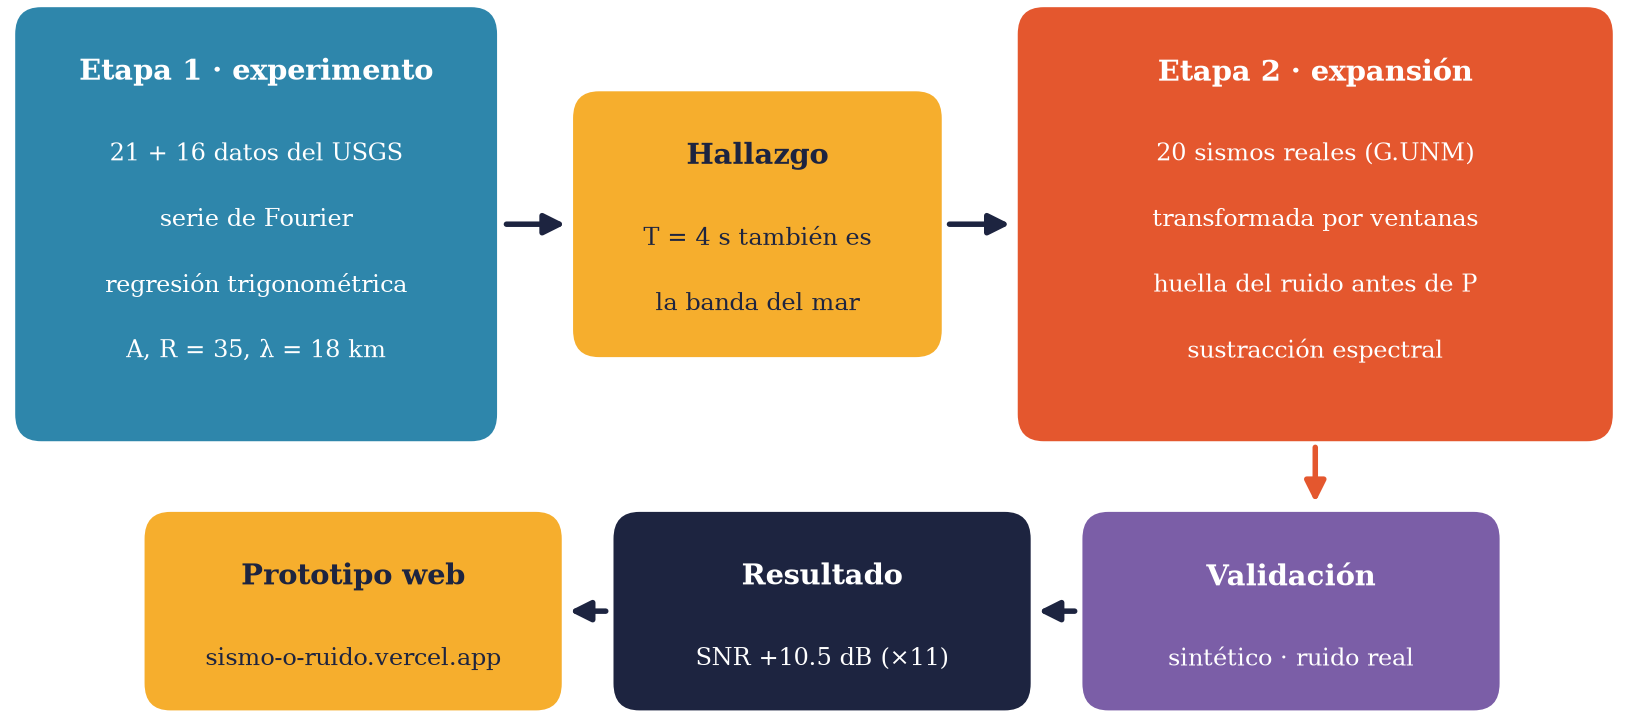
\includegraphics[width=0.95\textwidth]{enfoque.png}
\caption{Enfoque del proyecto. La etapa 1 prueba el modelo en un caso controlado y su límite motiva la etapa 2. \fuente}
\label{fig:enfoque}
\end{figure}

\textbf{Etapa 1.} Datos: dos registros simplificados del USGS en aceleración normalizada, uno cada $\Delta t = \SI{0.4}{s}$ (Tabla~\ref{tab:datos}). El del sensor tiene 21 datos durante un sismo y el ambiental 16 datos sin sismo. Procedimiento: serie de Fourier y Parseval (sección~7.1), regresión trigonométrica (7.2), energía y longitud de onda (7.3).

\textbf{Etapa 2.} Datos: 20 sismos de México con $M \geq 6.8$, de 1993 a 2026, del catálogo del USGS \parencite{comcat}. Se usa el canal vertical BHZ, 20 muestras por segundo, de la estación G.UNM en Ciudad Universitaria, descargado de EarthScope \parencite{geoscope} con ObsPy \parencite{obspy2010}. Se corrige la respuesta del instrumento para obtener velocidad, se deja la banda de 0.04 a \SI{8}{Hz} y se recorta de 5 minutos antes a 10 minutos después de la onda P. Procedimiento: transformada por ventanas (7.4 y 7.5), filtro de separación (7.6) y medición de la relación señal-ruido.

\textbf{Validación.} Identidades exactas (Parseval y DFT igual a serie), un sismo sintético de forma conocida y ruido real a distintos niveles mediante sustitutos de Fourier \parencite{theiler1992} (sección~9).

\textbf{Herramientas.} Python 3 con NumPy, SciPy, Matplotlib y ObsPy, verificación a mano de los cálculos de la etapa 1, \LaTeX{} para el reporte y un prototipo web que publica los resultados \parencite{prototipo}.

\begin{table}[H]
\centering
\small
\begin{tabular}{ccc@{\hspace{1.2cm}}ccc}
\toprule
$t$ (s) & Sensor & Ambiental & $t$ (s) & Sensor & Ambiental\\
\midrule
0.0 & 0.02 & 0.03 & 4.4 & $-0.04$ & 0.06\\
0.4 & 0.08 & 0.05 & 4.8 & 0.18 & 0.07\\
0.8 & 0.21 & 0.07 & 5.2 & 0.33 & 0.05\\
1.2 & 0.35 & 0.04 & 5.6 & 0.39 & 0.01\\
1.6 & 0.41 & 0.02 & 6.0 & 0.27 & $-0.03$\\
2.0 & 0.29 & $-0.01$ & 6.4 & 0.05 & --\\
2.4 & 0.10 & $-0.05$ & 6.8 & $-0.17$ & --\\
2.8 & $-0.12$ & $-0.06$ & 7.2 & $-0.34$ & --\\
3.2 & $-0.31$ & $-0.04$ & 7.6 & $-0.40$ & --\\
3.6 & $-0.38$ & $-0.01$ & 8.0 & $-0.22$ & --\\
4.0 & $-0.25$ & 0.03 & & & \\
\bottomrule
\end{tabular}
\caption{Registros simplificados del USGS en aceleración normalizada (límite de redondeo $\pm 0.005$).}
\label{tab:datos}
\end{table}

% ================= 6 MODELO =================
\section{Desarrollo del modelo matemático}
\subsection{Campo de desplazamiento y potenciales}
En un medio elástico, homogéneo e isótropo, el desplazamiento $\mathbf{u}$ cumple la ecuación de Navier \parencite{shearer2019}:
\begin{equation}
\rho\,\frac{\partial^2\mathbf{u}}{\partial t^2} = (\lambda_L + 2\mu)\,\nabla(\nabla\cdot\mathbf{u}) - \mu\,\nabla\times(\nabla\times\mathbf{u})
\label{eq:navier}
\end{equation}
donde $\lambda_L$ y $\mu$ son las constantes de Lamé en \si{Pa}. Por el teorema de Helmholtz, todo campo suave que decae en el infinito se escribe como el gradiente de un potencial escalar más el rotacional de un potencial vectorial:
\begin{equation}
\mathbf{u} = \nabla\phi + \nabla\times\boldsymbol{\psi}, \qquad \nabla\cdot\boldsymbol{\psi} = 0
\label{eq:helm}
\end{equation}
Al sustituir la Ec.~\eqref{eq:helm} en la Ec.~\eqref{eq:navier} y usar $\nabla\cdot(\nabla\times\boldsymbol\psi) = 0$ y $\nabla\times\nabla\phi = \mathbf{0}$, la ecuación se separa en dos ecuaciones de onda independientes:
\begin{equation}
\frac{\partial^2\phi}{\partial t^2} = v_P^2\,\nabla^2\phi, \quad v_P = \sqrt{\frac{\lambda_L + 2\mu}{\rho}}, \qquad
\frac{\partial^2\boldsymbol\psi}{\partial t^2} = v_S^2\,\nabla^2\boldsymbol\psi, \quad v_S = \sqrt{\frac{\mu}{\rho}}
\label{eq:PS}
\end{equation}
La parte $\nabla\phi$ tiene rotacional nulo y es la onda P, de compresión. La parte $\nabla\times\boldsymbol\psi$ tiene divergencia nula y es la onda S, de cortante. Como $\lambda_L > 0$, se cumple $v_P > v_S$, y por eso la P llega primero. Esa es la base física de la alerta temprana.

\subsection{Del potencial al armónico}
Si el campo oscila con frecuencia $\omega$, se escribe $\phi(\mathbf r,t) = \operatorname{Re}\{\Phi(\mathbf r)\,e^{i\omega t}\}$ con $\Phi$ complejo. Al sustituir en la Ec.~\eqref{eq:PS} se obtiene la ecuación de Helmholtz:
\begin{equation}
\nabla^2\Phi + k^2\Phi = 0, \qquad k = \frac{\omega}{v}
\label{eq:helmholtz}
\end{equation}
En el límite de longitud de onda muy grande, $k \to 0$, la Ec.~\eqref{eq:helmholtz} se reduce a la ecuación de Laplace, $\nabla^2\Phi = 0$. Sus soluciones son funciones armónicas, como en la teoría del potencial. En dos dimensiones, toda función armónica es la parte real de una función analítica $F(z) = \Phi + i\Psi$ con $z = x + iy$. En el otro extremo, $k$ finita, la Ec.~\eqref{eq:helmholtz} admite la onda plana $\Phi = U e^{-i\mathbf k\cdot\mathbf r}$, que es la que supone el modelo. En el sensor, fijo en $\mathbf r_0$, la onda plana se ve como una función armónica del tiempo, $u(t) = U\cos(\omega t + \varphi)$. Por eso la serie de Fourier, una suma de armónicos, es la herramienta natural para describir lo que registra.

\subsection{Modelo de la señal registrada}
El sensor mide aceleración, la segunda derivada del desplazamiento en un punto, más el ruido:
\begin{equation}
x(t) = s(t) + r(t), \qquad s(t) = \frac{\partial^2 u(\mathbf r_0, t)}{\partial t^2}
\label{eq:balance}
\end{equation}
En la etapa 1 cada término se aproxima con su componente dominante, una sola onda de frecuencia $\omega$:
\begin{equation}
x_i \approx c_x + a_x\cos\omega t_i + b_x\sin\omega t_i, \qquad r_j \approx c_r + a_r\cos\omega t_j + b_r\sin\omega t_j
\label{eq:modelo}
\end{equation}
En la etapa 2 el modelo se mantiene, pero cada término se describe con todo su contenido espectral en ventanas de tiempo, y la separación se hace en el plano tiempo-frecuencia (secciones~7.4 a 7.6).

% ================= 7 DESARROLLO MATEMÁTICO =================
\section{Desarrollo matemático completo}

\subsection{Serie de Fourier discreta, ortogonalidad y Parseval}
Sean $N$ datos $x_i$ tomados en $t_i = i\Delta t$, con $T_0 = N\Delta t$ y $\omega_0 = 2\pi/T_0$. Se buscan coeficientes tales que
\begin{equation}
x_i = \sum_{n=0}^{N-1} c_n\, e^{\,i n\omega_0 t_i} = \sum_{n=0}^{N-1} c_n\, W^{\,ni}, \qquad W = e^{\,i2\pi/N}
\label{eq:compleja}
\end{equation}
donde $W$ es una raíz $N$-ésima de la unidad, $W^N = 1$. Las potencias $W^m$ son los vértices de un polígono regular en el círculo unitario del plano complejo.

\begin{prop}[Ortogonalidad discreta]
Para enteros $m$ y $n$ entre $0$ y $N-1$,
\begin{equation}
\sum_{i=0}^{N-1} W^{\,(m-n)i} = N\,\delta_{mn}
\label{eq:ortog}
\end{equation}
\end{prop}
\textit{Demostración.} Si $m = n$, cada término vale 1 y la suma es $N$. Si $m \neq n$, sea $q = W^{m-n} \neq 1$. La suma es geométrica:
$\sum_{i=0}^{N-1} q^i = \dfrac{1 - q^N}{1 - q} = \dfrac{1 - W^{(m-n)N}}{1 - q} = \dfrac{1 - 1}{1 - q} = 0$. $\square$

Con los 21 datos del sensor, la suma numérica de $W^i$ da $3.7\times10^{-15}$, cero dentro del redondeo de la máquina. Al multiplicar la Ec.~\eqref{eq:compleja} por $W^{-mi}$, sumar sobre $i$ y usar la Ec.~\eqref{eq:ortog}, solo sobrevive el término $n = m$:
\begin{equation}
c_m = \frac{1}{N}\sum_{i=0}^{N-1} x_i\, W^{-mi} = \frac{X_m}{N}
\label{eq:cm}
\end{equation}
donde $X_m = \sum_i x_i e^{-i2\pi mi/N}$ es la transformada de Fourier discreta (DFT). Como $x_i$ es real, $c_{N-m} = \overline{c_m}$. Al agrupar los términos $m$ y $N-m$ y usar la fórmula de Euler $e^{i\theta} = \cos\theta + i\sin\theta$, se obtiene la forma real:
\begin{equation}
x_i = a_0 + \sum_{n\geq1}\left[a_n\cos(n\omega_0 t_i) + b_n\sin(n\omega_0 t_i)\right], \qquad
a_n = 2\operatorname{Re}c_n = \frac{2}{N}\sum_i x_i\cos(n\omega_0 t_i), \quad b_n = -2\operatorname{Im}c_n = \frac{2}{N}\sum_i x_i\sin(n\omega_0 t_i)
\label{eq:fourier}
\end{equation}
con $a_0 = c_0$ el promedio. La suma real llega hasta $n = (N-1)/2 = 10$ porque $N = 21$ es impar. El número complejo $c_n$ guarda la amplitud y la fase de cada armónico. Su módulo es la mitad de la amplitud y su argumento es la fase:
\begin{equation}
c_n = \frac{A_n}{2}\,e^{i\varphi_n}, \qquad A_n = \sqrt{a_n^2 + b_n^2} = 2|c_n|, \qquad \varphi_n = \operatorname{Arg}c_n = \operatorname{atan2}(-b_n, a_n)
\label{eq:Aphi}
\end{equation}
La función $\operatorname{atan2}$ es el argumento principal de un número complejo y elige el cuadrante correcto.

\begin{prop}[Parseval discreto]
\begin{equation}
\frac{1}{N}\sum_{i=0}^{N-1} |x_i|^2 = \sum_{n=0}^{N-1}|c_n|^2, \qquad\text{y por tanto}\qquad \sigma^2 = \sum_{n\geq1}\frac{A_n^2}{2}
\label{eq:parseval}
\end{equation}
\end{prop}
\textit{Demostración.} $\frac{1}{N}\sum_i |x_i|^2 = \frac1N\sum_i\sum_m\sum_n c_m\overline{c_n}\,W^{(m-n)i} = \sum_m\sum_n c_m\overline{c_n}\,\delta_{mn} = \sum_n |c_n|^2$, por la Ec.~\eqref{eq:ortog}. Al quitar el promedio ($n = 0$) y juntar los pares $n$, $N-n$, cada armónico real aporta $2|c_n|^2 = A_n^2/2$. $\square$

La Ec.~\eqref{eq:parseval} reparte la varianza entre los armónicos. La fracción de cada uno es
\begin{equation}
p_n = \frac{A_n^2}{2\sigma^2}, \qquad \sum_{n\geq1} p_n = 1
\label{eq:pn}
\end{equation}

\subsection{Regresión trigonométrica por mínimos cuadrados}
Para una frecuencia $\omega$ fija se busca el vector $\boldsymbol\beta = (c, a, b)^T$ que minimiza la suma de errores al cuadrado
\begin{equation}
S(\boldsymbol\beta) = \|\mathbf y - \mathbf M\boldsymbol\beta\|^2 = \sum_i\left[y_i - c - a\cos\omega t_i - b\sin\omega t_i\right]^2
\label{eq:S}
\end{equation}
donde cada fila de $\mathbf M$ es $(1, \cos\omega t_i, \sin\omega t_i)$. Como $S$ es una forma cuadrática convexa, su mínimo está donde el gradiente se anula, $\nabla_{\boldsymbol\beta} S = -2\mathbf M^T(\mathbf y - \mathbf M\boldsymbol\beta) = \mathbf 0$. De ahí salen las ecuaciones normales:
\begin{equation}
\left(\mathbf M^T\mathbf M\right)\boldsymbol\beta = \mathbf M^T\mathbf y
\label{eq:normal}
\end{equation}
El residuo $\mathbf e = \mathbf y - \mathbf M\boldsymbol\beta$ queda ortogonal a las columnas de $\mathbf M$. Geométricamente, la regresión es la proyección ortogonal de los datos sobre el espacio generado por $1$, $\cos\omega t$ y $\sin\omega t$. Si la ventana contuviera un número entero de periodos, la Ec.~\eqref{eq:ortog} haría $\mathbf M^T\mathbf M$ diagonal y la regresión coincidiría con la Ec.~\eqref{eq:fourier}. Con $T = \SI{4.0}{s}$ y 21 datos casi se cumple, y la matriz resulta casi diagonal (sección~8.1).

Con $s^2 = S_{\min}/(N-3)$ la varianza de los residuos, la matriz de covarianza de los parámetros y sus errores estándar son
\begin{equation}
\operatorname{Cov}(\boldsymbol\beta) = s^2\left(\mathbf M^T\mathbf M\right)^{-1}, \qquad \mathrm{EE}(\beta_k) = s\sqrt{\left[(\mathbf M^T\mathbf M)^{-1}\right]_{kk}}
\label{eq:ee}
\end{equation}
La amplitud $A = \sqrt{a^2 + b^2}$ es una función no lineal de $a$ y $b$. Su error se obtiene con la aproximación lineal de primer orden:
\begin{equation}
\delta A^2 = \left(\frac{a}{A}\right)^2\delta a^2 + \left(\frac{b}{A}\right)^2\delta b^2 + 2\,\frac{ab}{A^2}\operatorname{Cov}(a,b)
\label{eq:dA}
\end{equation}

\subsection{Energía de la onda, cociente de energías y longitud de onda}
Para una onda plana $u = U\cos(kx - \omega t)$ que cumple la ecuación de onda unidimensional, la densidad de energía cinética es $\tfrac12\rho\,u_t^2$ y la potencial elástica es $\tfrac12\rho v^2 u_x^2$. Al sustituir, con $u_t = U\omega\sin(kx-\omega t)$ y $u_x = -Uk\sin(kx-\omega t)$, y usar la relación de dispersión $\omega = vk$, que sale de sustituir la onda plana en la Ec.~\eqref{eq:PS}:
\begin{equation}
e = \tfrac12\rho U^2\omega^2\sin^2(kx-\omega t) + \tfrac12\rho v^2U^2k^2\sin^2(kx-\omega t) = \rho U^2\omega^2\sin^2(kx-\omega t)
\label{eq:e}
\end{equation}
Como el promedio de $\sin^2$ en un periodo es $\tfrac12$, la energía media por unidad de volumen es
\begin{equation}
\bar e = \tfrac12\rho\,\omega^2 U^2
\label{eq:energia}
\end{equation}
Los datos son aceleraciones. Para una onda armónica, $\ddot u = -\omega^2 u$, así que la amplitud de aceleración $A$ y la de desplazamiento $U$ cumplen $U = A/\omega^2$. Al combinar con la Ec.~\eqref{eq:energia}:
\begin{equation}
\bar e = \frac12\rho\,\omega^2\left(\frac{A}{\omega^2}\right)^2 = \frac{\rho A^2}{2\omega^2}
\label{eq:eA}
\end{equation}
Al dividir la energía del sensor entre la del ruido, con el mismo medio, se cancela $\rho$:
\begin{equation}
R = \frac{\bar e_x}{\bar e_r} = \left(\frac{A_x\,\omega_r}{A_r\,\omega_x}\right)^2 \;\xrightarrow{\ \omega_x = \omega_r\ }\; \left(\frac{A_x}{A_r}\right)^2, \qquad
\frac{\delta R}{R} = 2\sqrt{\left(\frac{\delta A_x}{A_x}\right)^2 + \left(\frac{\delta A_r}{A_r}\right)^2}
\label{eq:R}
\end{equation}
La segunda expresión es la propagación de errores relativos de un cociente elevado al cuadrado. Finalmente, la relación de dispersión con $k = 2\pi/\lambda$ y $\omega = 2\pi/T$ da la longitud de onda:
\begin{equation}
\omega = vk \;\Rightarrow\; \lambda = \frac{v}{f} = vT
\label{eq:lambda}
\end{equation}

\subsection{De la serie a la transformada integral de Fourier}
La serie de Fourier supone que la señal se repite con periodo $T_0$. Un registro sísmico real no es periódico. El sismo empieza y termina, y su contenido de frecuencias cambia con el tiempo. Para una señal de energía finita se toma el límite $T_0 \to \infty$ en la serie compleja. El espaciado de frecuencias $\Delta\omega = 2\pi/T_0$ tiende a $d\omega$, la suma se vuelve integral y los coeficientes $T_0 c_n$ se vuelven una función continua:
\begin{equation}
\hat x(f) = \int_{-\infty}^{\infty} x(t)\,e^{-i2\pi ft}\,dt, \qquad x(t) = \int_{-\infty}^{\infty}\hat x(f)\,e^{\,i2\pi ft}\,df
\label{eq:transformada}
\end{equation}
El teorema de Plancherel extiende Parseval al caso continuo, $\int|x|^2dt = \int|\hat x|^2df$, y la energía de la señal se reparte en frecuencia con la densidad $|\hat x(f)|^2$.

\textbf{Muestreo y Nyquist.} Muestrear cada $\Delta t$ equivale a multiplicar $x(t)$ por un tren de deltas. La transformada de ese tren es otro tren de deltas separado $1/\Delta t$, y por el teorema de convolución el espectro muestreado es la suma de copias de $\hat x$ desplazadas $1/\Delta t$. Las copias no se enciman solo si $\hat x(f) = 0$ para $|f| > f_N$, con
\begin{equation}
f_N = \frac{1}{2\Delta t}
\label{eq:nyquist}
\end{equation}
Con $\Delta t = \SI{0.4}{s}$, $f_N = \SI{1.25}{Hz}$. Con 20 muestras por segundo, $f_N = \SI{10}{Hz}$. Por eso en la etapa 2 se deja la banda de 0.04 a \SI{8}{Hz} antes de analizar.

\textbf{DFT.} Con $N$ muestras, la Ec.~\eqref{eq:transformada} se aproxima por la suma de la Ec.~\eqref{eq:cm}, $\hat x(k/T_0) \approx \Delta t\,X_k$. La DFT y la serie de Fourier discreta son el mismo objeto. Con los 21 datos, la DFT reproduce exactamente $a_0 = 0.0214$, $a_2 = -0.147$ y $b_2 = 0.333$. Se calcula con el algoritmo de \textcite{cooley1965}.

\subsection{Transformada por ventanas y fuga espectral}
Para seguir el cambio de frecuencias en el tiempo, la señal se multiplica por una ventana $w$ de duración $L$ centrada en $\tau$ y se transforma:
\begin{equation}
X(\tau, f) = \int x(t)\,w(t - \tau)\,e^{-i2\pi ft}\,dt, \qquad X(m,k) = \sum_{i=0}^{L-1} x_{i+mH}\,w_i\,e^{-i2\pi ki/L}
\label{eq:stft}
\end{equation}
La segunda forma es la discreta, con salto $H$ entre ventanas. Por el teorema de convolución, el producto $x\cdot w$ en el tiempo es una convolución en frecuencia:
\begin{equation}
\widehat{x\,w}(f) = (\hat x * \hat w)(f) = \int \hat x(\nu)\,\hat w(f - \nu)\,d\nu
\label{eq:convolucion}
\end{equation}
Cada línea espectral se ve ensanchada con la forma de $\hat w$. Ese ensanchamiento es la fuga espectral. Una ventana rectangular tiene lóbulos laterales que caen lento, como $1/f$. La ventana de Hann, $w_i = \sin^2(\pi i/L)$, los hace caer como $1/f^3$ a cambio de un lóbulo principal de ancho $4/L$. La resolución en frecuencia es $\Delta f = 1/L$. Con $L = \SI{25.6}{s}$ (512 datos), $\Delta f = \SI{0.039}{Hz}$ y el lóbulo principal mide \SI{0.16}{Hz}. Eso alcanza para resolver el pico de microsismos entre 0.1 y \SI{0.35}{Hz}. Con traslape de \SI{75}{\percent}, la suma de ventanas de Hann es constante y la transformada inversa reconstruye la señal sin distorsión. El mapa $|X(m,k)|^2$ es el espectrograma.

\subsection{Separación de sismo y ruido: del filtro de Wiener a la sustracción espectral}
Por la linealidad de la Ec.~\eqref{eq:stft}, en cada celda $X = S + R$. Se busca una ganancia real $G$ que haga $\hat S = G X$ lo más parecida posible a $S$ en el sentido de mínimo error cuadrático medio:
\begin{equation}
J(G) = \mathbb E\left[|S - GX|^2\right] = \mathbb E|S|^2 - 2G\,\mathbb E[\operatorname{Re}(\overline S X)] + G^2\,\mathbb E|X|^2
\label{eq:J}
\end{equation}
Si $S$ y $R$ no están correlacionados, $\mathbb E[\overline S X] = \mathbb E|S|^2$ y $\mathbb E|X|^2 = \mathbb E|S|^2 + \mathbb E|R|^2$. Al derivar e igualar a cero, $dJ/dG = 0$:
\begin{equation}
G_{\text{Wiener}} = \frac{\mathbb E|S|^2}{\mathbb E|S|^2 + \mathbb E|R|^2} = 1 - \frac{\mathbb E|R|^2}{\mathbb E|X|^2}
\label{eq:wiener}
\end{equation}
Esta es la ganancia de Wiener. Siempre está entre 0 y 1. Vale casi 1 donde domina el sismo y casi 0 donde domina el ruido. El problema práctico es que $\mathbb E|R|^2$ no se conoce. La física de la alerta da la solución. Antes de la onda P solo hay ruido, así que su potencia se estima promediando las $M$ ventanas previas \parencite{boll1979,mousavi2016}:
\begin{equation}
P_R(k) = \frac{1}{M}\sum_{m\,\in\,\text{ruido}}|X(m,k)|^2
\label{eq:pruido}
\end{equation}
Al sustituir $\mathbb E|R|^2 \approx P_R(k)$ y $\mathbb E|X|^2 \approx |X(m,k)|^2$ en la Ec.~\eqref{eq:wiener}, y tomar raíz para aplicar la ganancia a la amplitud, se obtiene la sustracción espectral de potencia con sobresustracción $\beta$ y piso $g_{\min}$ \parencite{berouti1979}:
\begin{equation}
G(m,k) = \sqrt{\max\!\left(1 - \beta\,\frac{P_R(k)}{|X(m,k)|^2},\ g_{\min}^2\right)}
\label{eq:ganancia}
\end{equation}
El factor $\beta = 2$ compensa la variabilidad de $|X|^2$ alrededor de su media, y el piso $g_{\min} = 0.02$ evita ganancias exactamente nulas, que producen artefactos. La señal limpia es $\hat s = \text{STFT}^{-1}\{G X\}$, conservando la fase de $X$, y el ruido estimado es $\hat r = x - \hat s$. Para no mezclar el sismo en la Ec.~\eqref{eq:pruido}, solo se usan ventanas que terminan \SI{40}{s} antes de la onda P.

La calidad se mide con la relación señal-ruido entre una ventana con sismo y una sin él:
\begin{equation}
\mathrm{SNR} = 10\log_{10}\frac{\overline{s^2}_{\text{sismo}}}{\overline{s^2}_{\text{ruido}}}
\label{eq:snr}
\end{equation}
Cada \SI{10}{dB} multiplican por 10 la potencia. Se mide en los 3 minutos después de la P y en sus primeros \SI{10}{s}, los que usa una alerta temprana.

% ================= 8 RESULTADOS E INTERPRETACIÓN =================
\section{Resultados e interpretación física}

\subsection{Etapa 1. Serie de Fourier, regresión y energía}
Con los 21 datos del sensor, $T_0 = \SI{8.4}{s}$, $a_0 = 0.021$ y $\sigma^2 = 0.06984$. La Tabla~\ref{tab:fourier} y la Figura~\ref{fig:espectro} muestran los coeficientes. El segundo armónico, de periodo \SI{4.2}{s}, concentra el \SI{94.8}{\percent} de la varianza. La suma de los diez valores de $p_n$ da exactamente 1, como exige la Ec.~\eqref{eq:pn}. En forma compleja, $c_2 = -0.0737 - 0.1663\,i$, con $|c_2| = 0.182 = A_2/2$ y $\operatorname{Arg}c_2 = \SI{-1.99}{rad}$.

\begin{table}[H]
\centering
\small
\begin{tabular}{ccrrrcr}
\toprule
$n$ & $f_n$ (Hz) & $T_n$ (s) & $a_n$ & $b_n$ & $A_n$ & $p_n$ (\%)\\
\midrule
1 & 0.119 & 8.40 & 0.008 & 0.041 & 0.042 & 1.3\\
\textbf{2} & \textbf{0.238} & \textbf{4.20} & $\mathbf{-0.147}$ & \textbf{0.333} & \textbf{0.364} & \textbf{94.8}\\
3 & 0.357 & 2.80 & 0.047 & $-0.034$ & 0.058 & 2.4\\
4 & 0.476 & 2.10 & 0.031 & $-0.007$ & 0.031 & 0.7\\
5 & 0.595 & 1.68 & 0.018 & $-0.008$ & 0.019 & 0.3\\
6 & 0.714 & 1.40 & 0.024 & $-0.00049$ & 0.024 & 0.4\\
7--10 & & & & & $\leq 0.008$ & $< 0.1$ c/u\\
\bottomrule
\end{tabular}
\caption{Coeficientes de Fourier del registro del sensor, Ecs.~\eqref{eq:fourier} a \eqref{eq:pn}.}
\label{tab:fourier}
\end{table}

\textit{Sustitución:} $a_2 = \frac{2}{21}\sum x_i\cos(2\omega_0 t_i) = \frac{2}{21}(-1.548) = -0.147$ y $p_2 = A_2^2/(2\sigma^2) = 0.364^2/(2 \cdot 0.0698) = 0.948$.

\begin{figure}[H]
\centering
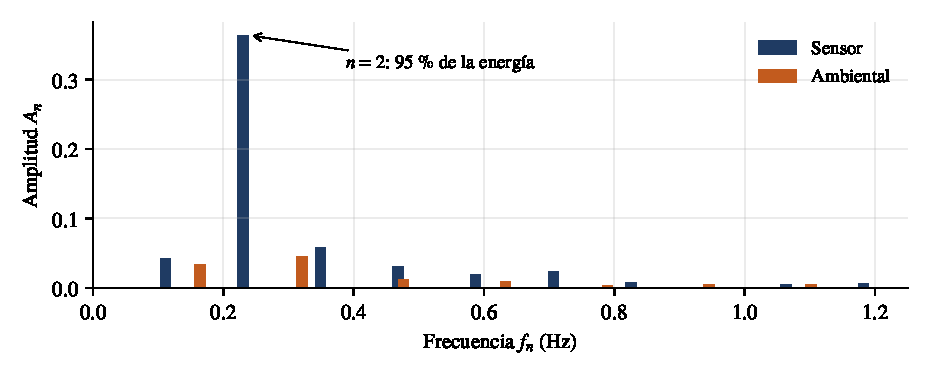
\includegraphics[width=0.78\textwidth]{espectro.pdf}
\caption{Amplitud de cada armónico de ambos registros. \fuente}
\label{fig:espectro}
\end{figure}

La distancia entre crestas es de \SI{4.0}{s} en ambos registros, así que se fija $\omega = 2\pi/\SI{4.0}{s} = \SI{1.571}{rad/s}$. Para el sensor, las ecuaciones normales son
\[
\begin{pmatrix} 21 & 1 & 0\\ 1 & 11 & 0\\ 0 & 0 & 10 \end{pmatrix}
\begin{pmatrix} c_x\\ a_x\\ b_x \end{pmatrix} =
\begin{pmatrix} 0.450\\ -2.578\\ 2.776 \end{pmatrix}
\]
La matriz es casi diagonal, como se anticipó en la sección~7.2. Los ceros en el bloque de $b$ aparecen porque $\sum\sin\omega t_i = 0$ y $\sum\cos\omega t_i\sin\omega t_i = 0$ en esta ventana. Al resolver, $b_x = 0.278$, $a_x = -0.237$, $c_x = 0.033$ y $A_x = \sqrt{0.237^2 + 0.278^2} = 0.365$. La Tabla~\ref{tab:ajuste} resume ambos registros.

\begin{table}[H]
\centering
\small
\begin{tabular}{lcccccc}
\toprule
Registro & $c$ & $a$ & $b$ & $A$ & $\varphi$ (rad) & $R^2$\\
\midrule
Sensor & $0.033 \pm 0.015$ & $-0.237 \pm 0.020$ & $0.278 \pm 0.021$ & $0.365 \pm 0.021$ & $-2.28$ & 0.95\\
Ambiental & $0.004 \pm 0.002$ & $0.026 \pm 0.002$ & $0.056 \pm 0.002$ & $0.062 \pm 0.002$ & $-1.14$ & 0.98\\
\bottomrule
\end{tabular}
\caption{Regresión trigonométrica con $T = \SI{4.0}{s}$, Ecs.~\eqref{eq:normal} a \eqref{eq:dA}.}
\label{tab:ajuste}
\end{table}

\begin{figure}[H]
\centering
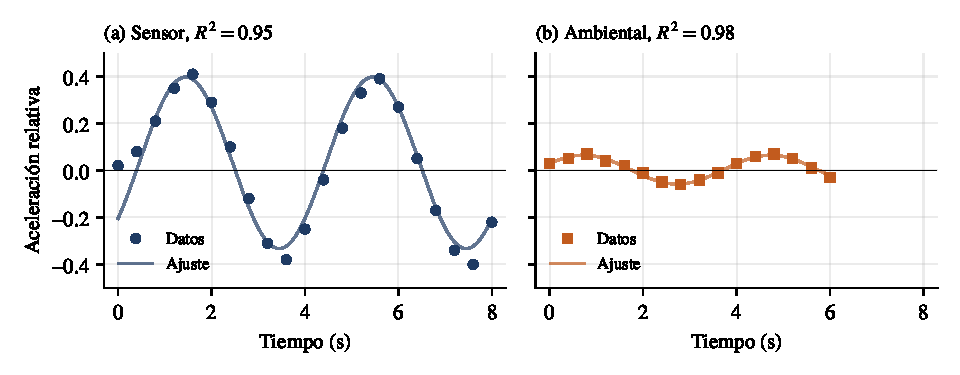
\includegraphics[width=0.82\textwidth]{ajuste.pdf}
\caption{Ajuste de una onda a cada registro del USGS. \fuente}
\label{fig:ajuste}
\end{figure}

Con la Ec.~\eqref{eq:R}, $R = (0.365/0.062)^2 = 35$ y $\delta R/R = 2\sqrt{(0.021/0.365)^2 + (0.002/0.062)^2} = 0.13$, así que $R = 35 \pm 5$. La hipótesis 1 se cumple. Con la Ec.~\eqref{eq:lambda}, $\lambda = (\SI{4500}{m/s})(\SI{4.0}{s}) = \SI{18000}{m}$ y $k = 2\pi/\lambda = \SI{3.5e-4}{rad/m}$. La amplitud de desplazamiento del sensor es $U = A/\omega^2 = 0.365/1.571^2 = 0.148$ en las mismas unidades normalizadas.

\textbf{Interpretación física.} Que un solo armónico explique el \SI{94.8}{\percent} de la varianza significa que, en esta ventana, el sensor registra prácticamente una onda plana monocromática, como predice la Ec.~\eqref{eq:helmholtz} lejos de la fuente. Como la energía escala con $A^2$, una amplitud 5.9 veces mayor se vuelve 35 veces más energía. Ese cuadrado es lo que hace detectable un sismo moderado sobre el ruido. La longitud de onda de \SI{18}{km} es del orden de la profundidad de \SI{15}{km}. A esa escala, el sensor no distingue detalles de la estructura y la aproximación de medio homogéneo es razonable. La fase $\varphi_x = \SI{-2.28}{rad}$ frente a $\varphi_r = \SI{-1.14}{rad}$ no tiene interpretación causal, porque los registros vienen de estaciones y momentos distintos.

\textbf{Lo que deja abierto la etapa 1.} Los dos registros tienen el mismo periodo de \SI{4}{s}, que cae en la banda de los microsismos. La diferencia está en la amplitud, no en la frecuencia. Además, con $f_N = \SI{1.25}{Hz}$ no se observa la energía de alta frecuencia de los sismos pequeños \parencite{brune1970}. Estas dos limitaciones motivan la etapa 2.

\subsection{Etapa 2. Registros reales}
La Figura~\ref{fig:registro} muestra el sismo de Puebla-Morelos de 2017 visto desde Ciudad Universitaria, a \SI{113}{km}. El registro crudo se separa en sismo y ruido. Antes de la onda P, el sismo separado queda casi en cero, como exige $G \to g_{\min}$ cuando $|X|^2 \approx P_R$.

\begin{figure}[H]
\centering
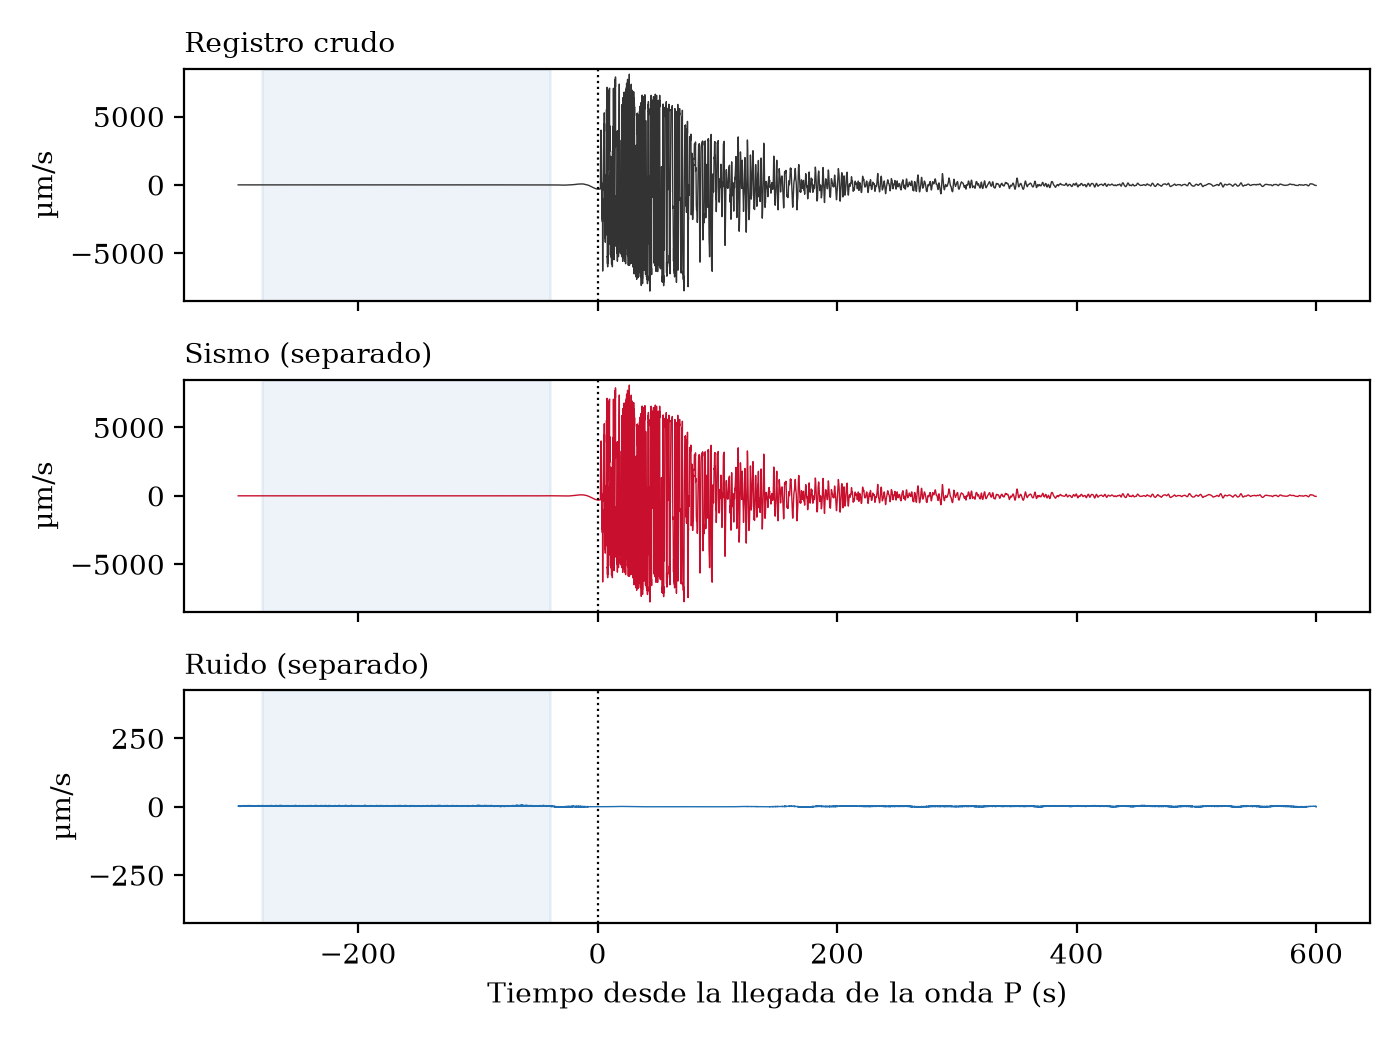
\includegraphics[width=0.85\textwidth]{real_registro.png}
\caption{Sismo de Puebla-Morelos (19 de septiembre de 2017, $M$ 7.1) en G.UNM. La franja azul es la ventana de ruido. Fuente: elaboración propia con datos del USGS y EarthScope.}
\label{fig:registro}
\end{figure}

La Figura~\ref{fig:espectro2} compara la transformada de la ventana del sismo con la de ruido. La Figura~\ref{fig:peterson} ubica el ruido entre los modelos de \textcite{peterson1993}, con la densidad espectral de Welch \parencite{welch1967}.

\begin{figure}[H]
\centering
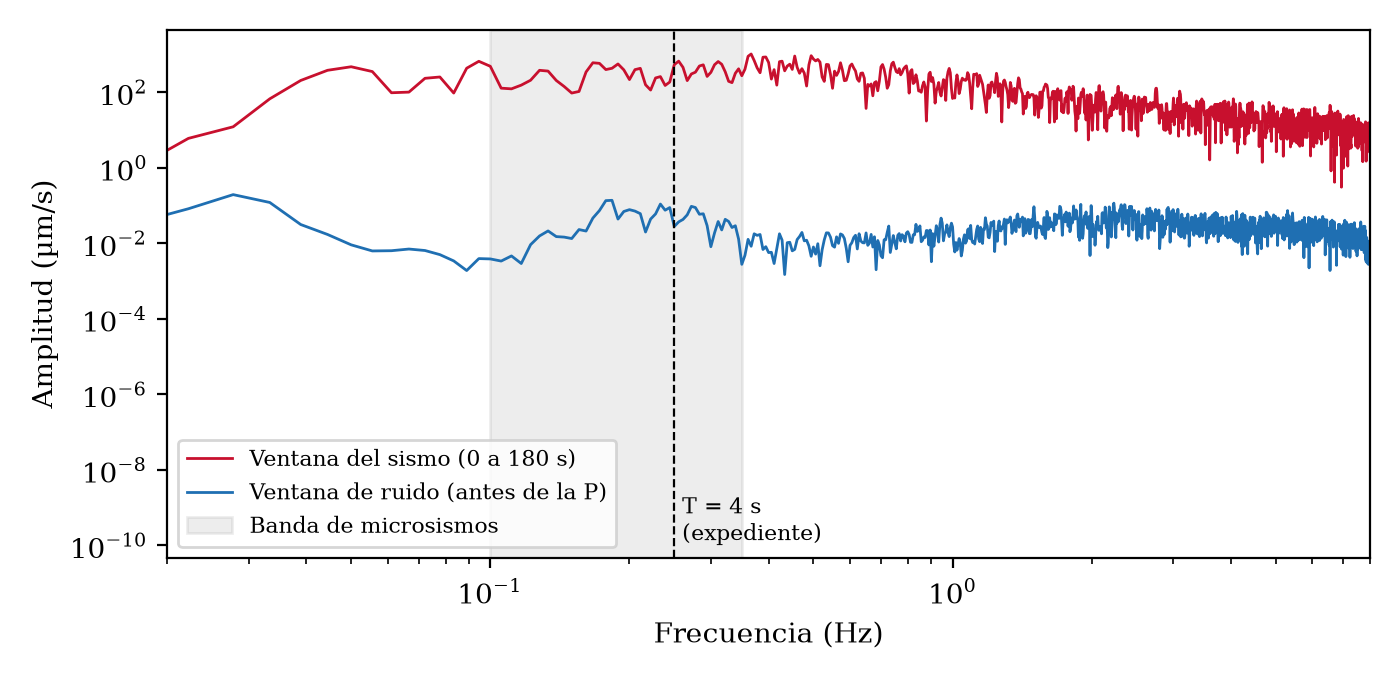
\includegraphics[width=0.82\textwidth]{real_espectro.png}
\caption{Espectro de amplitud del sismo de Puebla-Morelos y del ruido previo. La línea punteada marca el periodo de \SI{4}{s} de la etapa 1. \fuente}
\label{fig:espectro2}
\end{figure}

\begin{figure}[H]
\centering
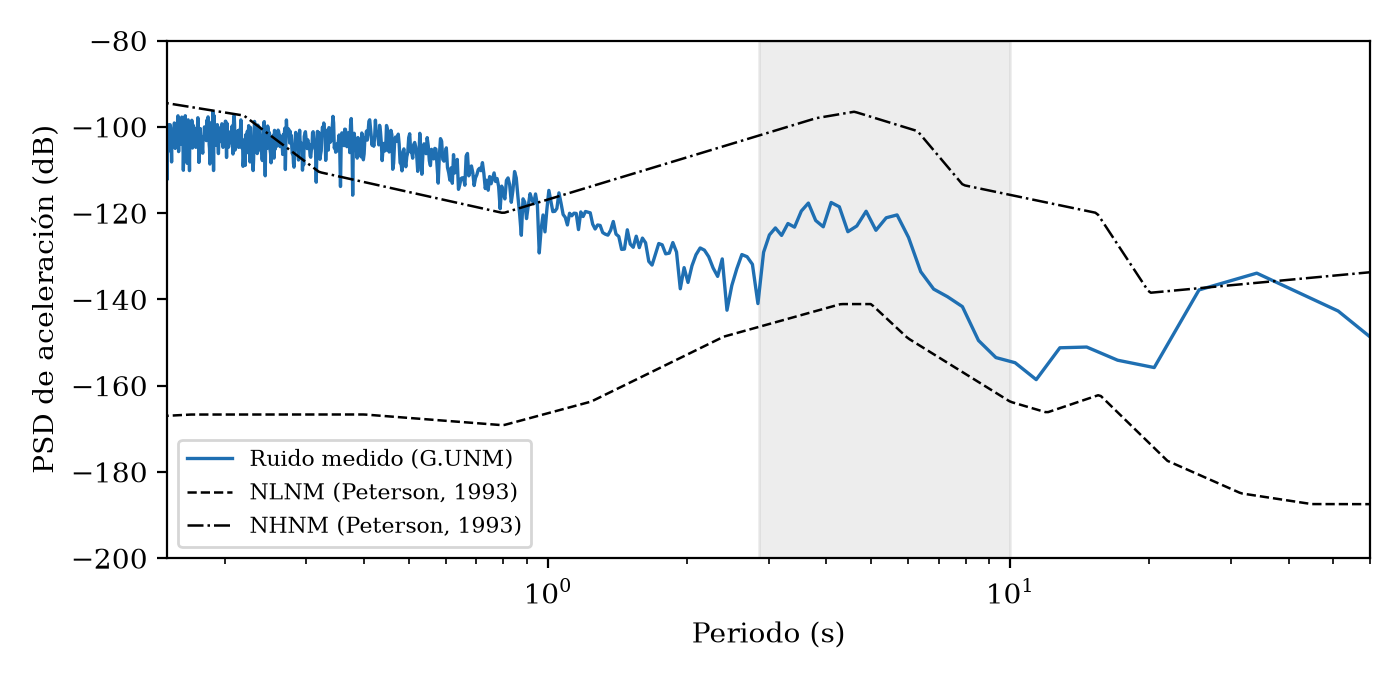
\includegraphics[width=0.82\textwidth]{real_peterson.png}
\caption{Densidad espectral del ruido de G.UNM frente a los modelos de ruido mínimo (NLNM) y máximo (NHNM). La franja gris es la banda de microsismos. \fuente}
\label{fig:peterson}
\end{figure}

\textbf{Interpretación física del ruido.} En los 20 sismos, el pico de microsismos tiene una mediana de \SI{6.4}{s}, con un rango de 3.0 a \SI{9.6}{s}. El mecanismo de \textcite{longuet1950} lo explica. Dos trenes de olas de frecuencia $f_o$ que viajan en sentidos opuestos forman una onda estacionaria. La presión en el fondo del mar depende del cuadrado de la elevación, y $\cos^2(2\pi f_o t) = \tfrac12[1 + \cos(4\pi f_o t)]$ oscila al doble de la frecuencia. Así, un pico de \SI{6.4}{s} corresponde a oleaje de unos \SI{12.8}{s}, típico de las marejadas del Pacífico. Por debajo de \SI{1}{s}, el ruido rebasa el modelo de ruido alto de Peterson. Ese es el ruido urbano de la Ciudad de México. Solo el \SI{14}{\percent} de la energía del ruido cae en la banda de microsismos, y el resto queda fuera de ella, sobre todo en las frecuencias altas del ruido urbano. Esto confirma el límite de la etapa 1. El ruido real sí tiene energía en la banda de \SI{4}{s}, y una separación solo por frecuencia la confundiría con un sismo.

La Figura~\ref{fig:espectrograma} muestra el espectrograma antes y después de aplicar la Ec.~\eqref{eq:ganancia}. La zona previa a la onda P se apaga y el sismo queda igual, porque ahí $|X|^2 \gg P_R$ y $G \approx 1$.

\begin{figure}[H]
\centering
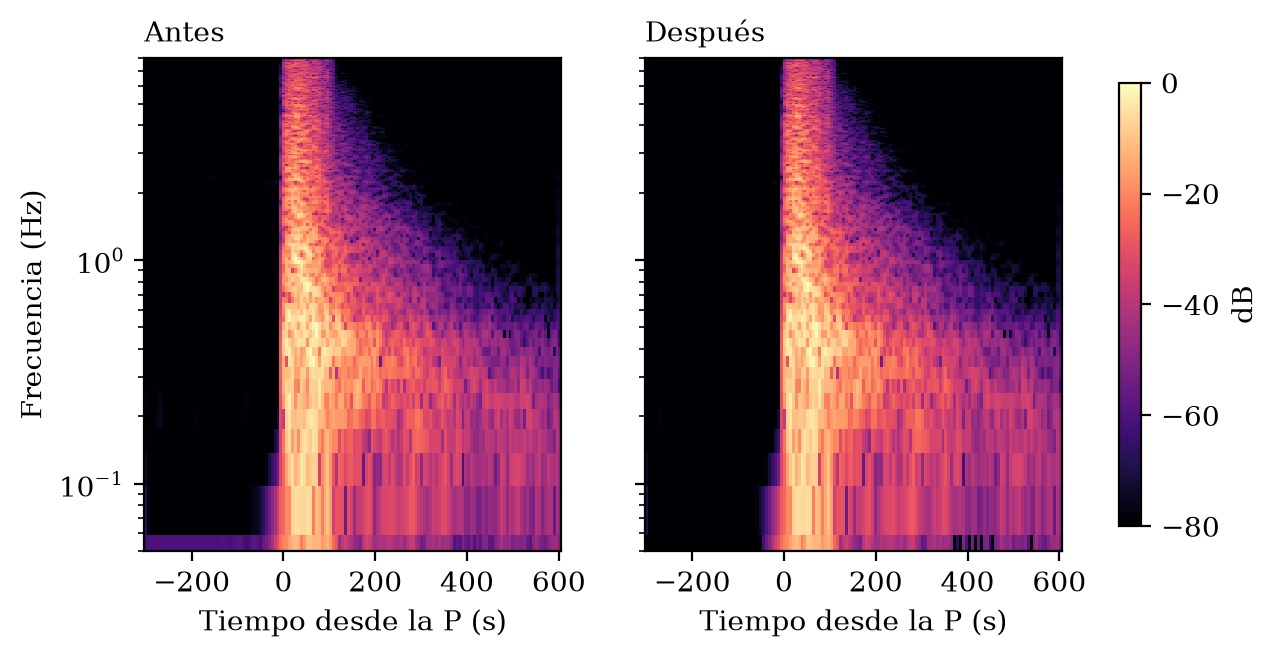
\includegraphics[width=0.82\textwidth]{real_espectrograma.png}
\caption{Espectrograma del sismo de Puebla-Morelos antes y después de la separación. \fuente}
\label{fig:espectrograma}
\end{figure}

La Tabla~\ref{tab:sismos} y la Figura~\ref{fig:resumen} resumen los 20 sismos. La SNR subió en todos, de 3.3 a \SI{17.6}{dB}, con un promedio de \SI{10.5}{dB}, unas 11 veces más potencia. En los primeros \SI{10}{s} de la P, la mejora promedio es de \SI{10.0}{dB}. La hipótesis 2 se cumple. El caso más difícil es el del Golfo de California de 2012. A \SI{1754}{km}, su onda P llega atenuada y casi no se distingue del ruido.

{\small\begin{longtable}{lcccccccc}
\toprule
Sismo & Fecha & $M$ & $d$ (km) & \multicolumn{2}{c}{SNR (dB)} & \multicolumn{2}{c}{SNR 10 s de P (dB)} & $T_{\text{mar}}$ (s)\\
\cmidrule(lr){5-6}\cmidrule(lr){7-8}
 & & & & antes & después & antes & después & \\
\midrule\endhead
Chiapas 1993 & 1993-09-10 & 7.2 & 863 & 39.8 & 50.0 & 13.3 & 22.9 & 9.6\\
Copala 1995 & 1995-09-14 & 7.4 & 289 & 61.5 & 76.4 & 43.1 & 58.1 & 3.9\\
Chiapas 1995 & 1995-10-21 & 7.2 & 664 & 50.6 & 61.7 & 35.6 & 46.6 & 5.6\\
Michoacán 1997 & 1997-01-11 & 7.2 & 397 & 66.3 & 74.5 & 41.2 & 49.4 & 4.4\\
Tehuacán 1999 & 1999-06-15 & 7.0 & 211 & 65.4 & 75.5 & 54.6 & 64.7 & 7.5\\
Oaxaca 1999 & 1999-09-30 & 7.5 & 433 & 47.8 & 58.8 & 36.5 & 47.6 & 3.5\\
Tecomán 2003 & 2003-01-22 & 7.6 & 522 & 67.0 & 77.2 & 39.5 & 49.7 & 6.9\\
El Mayor-Cucapah 2010 & 2010-04-04 & 7.2 & 2\,156 & 35.7 & 45.7 & 9.8 & 19.2 & 6.0\\
Ometepec 2012 & 2012-03-20 & 7.4 & 330 & 62.8 & 80.3 & 46.0 & 63.4 & 7.1\\
Golfo de California 2012 & 2012-04-12 & 7.0 & 1\,754 & 8.2 & 16.7 & -2.1 & -1.5 & 9.6\\
Papanoa 2014 & 2014-04-18 & 7.2 & 286 & 57.2 & 60.5 & 38.7 & 42.0 & 3.0\\
Chiapas 2014 & 2014-07-07 & 6.9 & 878 & 55.0 & 63.7 & 32.6 & 41.3 & 7.7\\
Tehuantepec 2017 & 2017-09-08 & 8.2 & 736 & 75.1 & 81.5 & 39.0 & 45.3 & 3.7\\
Puebla-Morelos 2017 & 2017-09-19 & 7.1 & 113 & 59.8 & 77.4 & 59.7 & 77.3 & 5.6\\
Pinotepa 2018 & 2018-02-16 & 7.2 & 350 & 64.5 & 76.7 & 39.6 & 51.8 & 6.7\\
Huatulco 2020 & 2020-06-23 & 7.4 & 508 & 68.0 & 81.4 & 42.4 & 55.7 & 7.5\\
Acapulco 2021 & 2021-09-08 & 7.0 & 271 & 72.8 & 80.3 & 59.2 & 66.7 & 7.3\\
Michoacán 2022 & 2022-09-19 & 7.6 & 410 & 68.2 & 78.9 & 28.7 & 39.4 & 8.0\\
Réplica Michoacán 2022 & 2022-09-22 & 6.8 & 415 & 71.9 & 80.1 & 45.9 & 54.2 & 6.2\\
Chiapas 2026 & 2026-07-17 & 7.3 & 846 & 45.6 & 55.2 & 22.4 & 31.9 & 6.0\\
\midrule
Promedio & & & & 57.2 & 67.6 & 36.3 & 46.3 & 6.4\textsuperscript{a}\\
\bottomrule
\caption{Resultados del método en los 20 sismos, registrados en la estación G.UNM. $d$ es la distancia epicentral y $T_{\text{mar}}$ el periodo del pico de microsismos del ruido. \textsuperscript{a}Mediana.}
\label{tab:sismos}
\end{longtable}}

\begin{figure}[H]
\centering
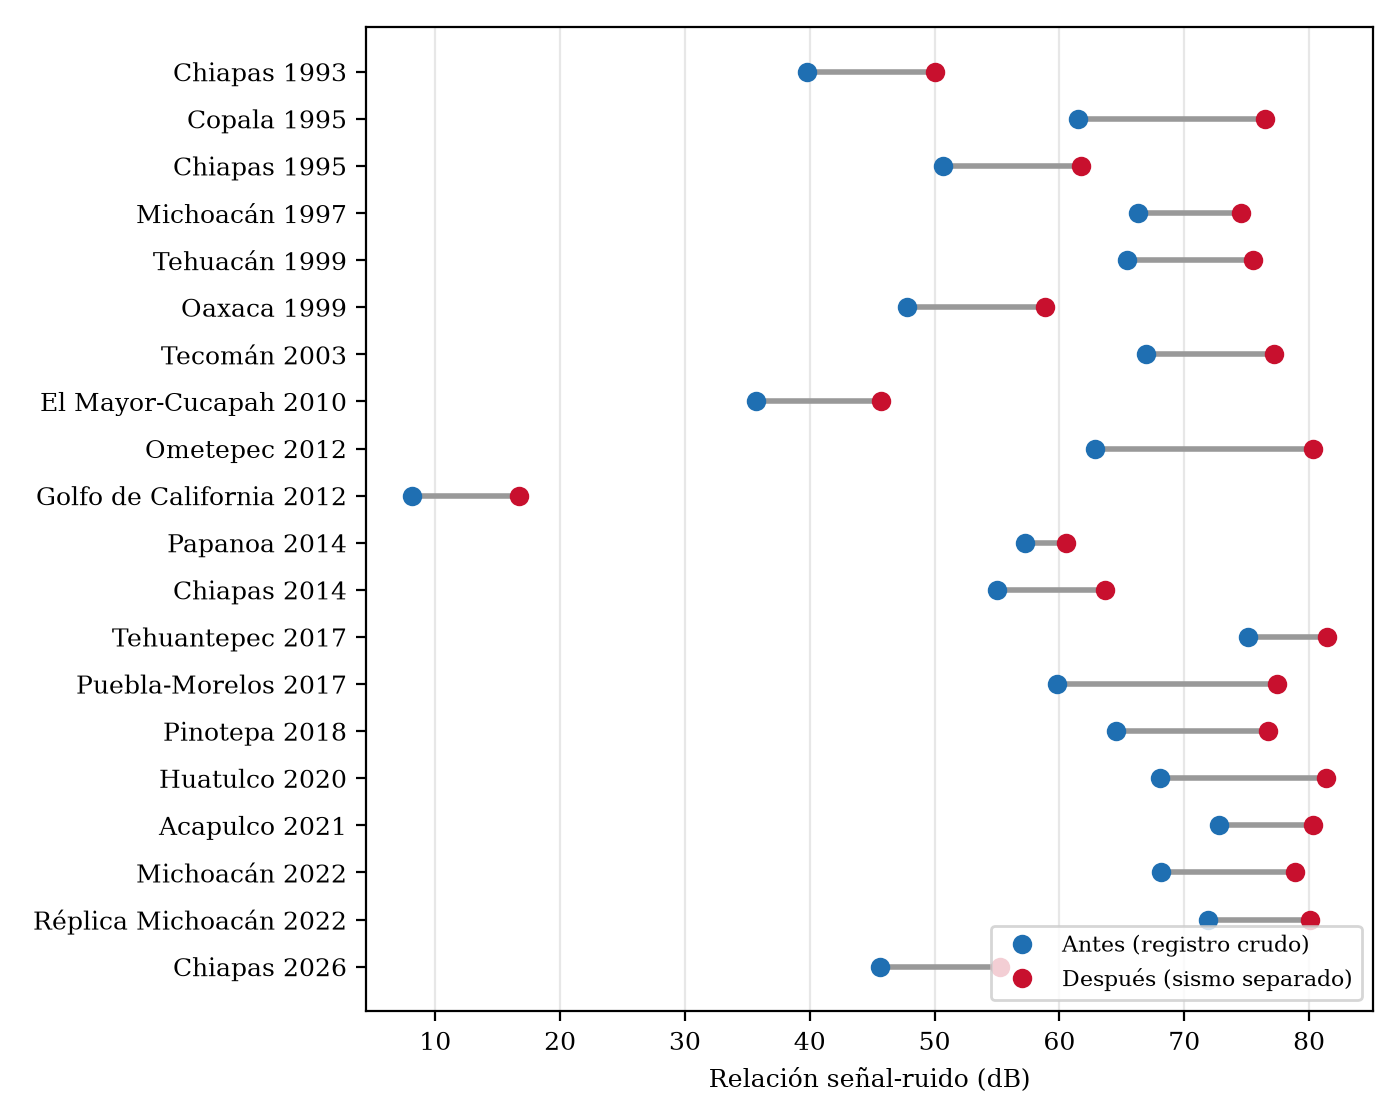
\includegraphics[width=0.75\textwidth]{real_resumen.png}
\caption{Relación señal-ruido de cada sismo antes y después de la separación. \fuente}
\label{fig:resumen}
\end{figure}

\textbf{Significado ingenieril.} Una mejora de \SI{10}{dB} en los primeros segundos de la P significa que la onda que dispara la alerta sobresale diez veces más sobre el ruido. Con un umbral fijo de detección, eso reduce las falsas alarmas o permite bajar el umbral y detectar antes. La ganancia de la Ec.~\eqref{eq:ganancia} es una regla local en cada celda tiempo-frecuencia, y su costo es el de una transformada rápida, $O(L\log L)$ por ventana. Por eso puede correr en tiempo real en equipos modestos.

% ================= 9 VALIDACIÓN =================
\section{Validación del modelo}
El modelo se validó en cuatro niveles.

\textbf{1. Identidades matemáticas.} La suma de las raíces de la unidad da $3.7\times10^{-15}$, la DFT reproduce todos los coeficientes de la Ec.~\eqref{eq:fourier} y Parseval se cumple con igualdad. La varianza calculada en el tiempo y en la frecuencia vale 0.069841 en ambos casos.

\textbf{2. Bondad de ajuste.} La regresión explica el \SI{94.6}{\percent} de la variación del sensor y el \SI{98.3}{\percent} de la del ruido. Los residuos son ortogonales a las columnas de $\mathbf M$, como exige la Ec.~\eqref{eq:normal}.

\textbf{3. Caso sintético.} Se construyó un registro con un microsismo de \SI{0.2}{Hz} con amplitud variable, ruido blanco y un sismo de 1.2 y \SI{2.5}{Hz} que empieza en un instante conocido. La separación recupera el sismo con una correlación de 0.996 y su SNR pasa de 5.9 a \SI{22.5}{dB}.

\textbf{4. Ruido real a distintos niveles.} A cada sismo limpio se le sumó ruido real alargado con sustitutos de Fourier, que conservan $|\hat r(f)|$ y cambian las fases al azar \parencite{theiler1992}. La Figura~\ref{fig:robustez} muestra el resultado. Con ruido tan fuerte como el sismo (\SI{0}{dB}), la correlación con la onda verdadera sube de 0.71 a 0.86. Con ruido tres veces más fuerte (\SI{-5}{dB}), sube de 0.48 a 0.67. Por encima de \SI{10}{dB} el filtro no daña la señal, porque $G \to 1$.

\begin{figure}[H]
\centering
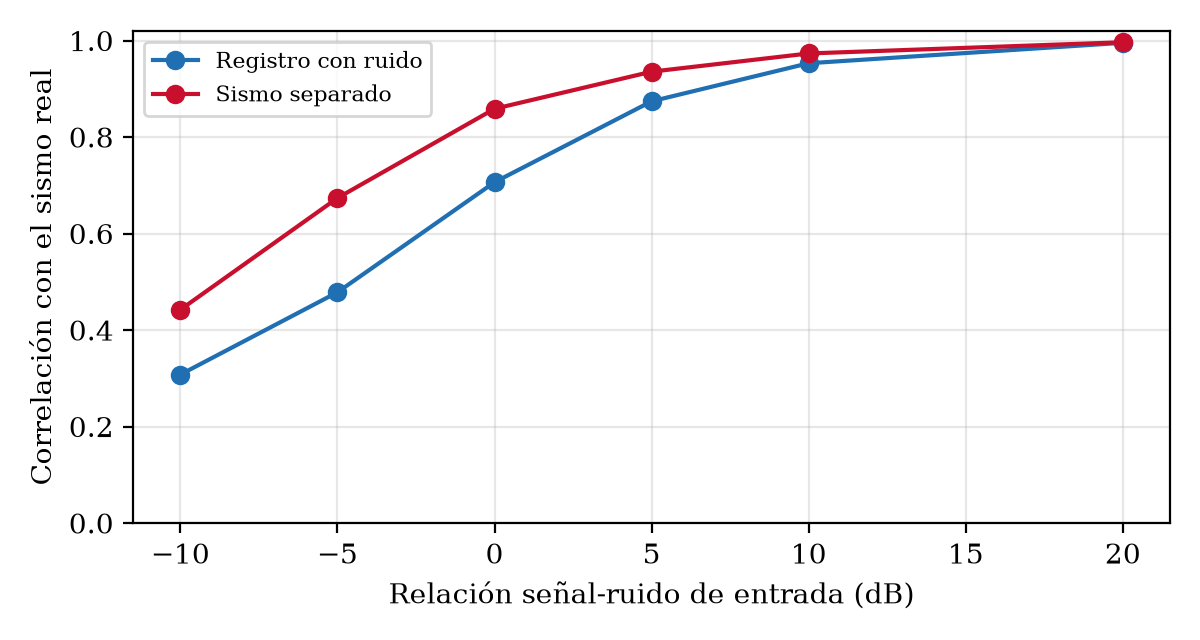
\includegraphics[width=0.7\textwidth]{real_robustez.png}
\caption{Correlación con el sismo real antes y después de separar, para distintos niveles de ruido real. Promedio de los 20 sismos. \fuente}
\label{fig:robustez}
\end{figure}

% ================= 10 DISCUSIÓN =================
\section{Discusión de resultados}
\textbf{Las dos etapas se complementan.} La etapa 1 cuantificó con números exactos que el sismo tiene unas 35 veces más energía que el ruido, pero mostró que la diferencia está en la amplitud y no en la frecuencia. La etapa 2 confirmó con datos reales que el mar produce ruido justo en esa banda. La serie de Fourier responde qué frecuencias hay. La transformada por ventanas responde además cuándo, y esa información temporal es la que permite separar.

\textbf{Interpretación del cociente $R$.} El valor de 35 compara componentes ajustadas bajo los supuestos del modelo. No dice qué porcentaje del sensor es sismo, porque el registro ambiental viene de otra estación y otro momento. En la etapa 2 esa limitación desaparece, porque el ruido se mide en la misma estación minutos antes.

\textbf{Relación con el estado del arte.} La Ec.~\eqref{eq:wiener} es la misma máscara que aprenden las redes de \textcite{zhu2019}, pero aquí sale de un principio de mínimo error y de una hipótesis física sobre el ruido. Eso la hace explicable y barata. A cambio, supone ruido estacionario, mientras que una red aprende ruido variable.

\textbf{Ondas P y S.} La separación en potenciales de la Ec.~\eqref{eq:helm} explica por qué la P llega primero y por qué su llegada marca el fin de la ventana de ruido. Con un solo sensor vertical no se pueden medir $\nabla\cdot\mathbf u$ ni $\nabla\times\mathbf u$, así que la separación P/S es teórica. Con un arreglo de sensores sí podría hacerse.

% ================= 11 LIMITACIONES =================
\section{Limitaciones}
\begin{itemize}
\item \textbf{Etapa 1.} Los registros son cortos (21 y 16 datos), con $f_N = \SI{1.25}{Hz}$, vienen de estaciones y momentos distintos y se supone la misma escala. El valor $\pm 0.005$ es límite de redondeo, no incertidumbre instrumental.
\item \textbf{Modelo físico.} Se supone medio homogéneo y onda plana. La longitud de onda de \SI{18}{km} es comparable con la profundidad, así que los efectos de capas y de sitio quedan fuera.
\item \textbf{Etapa 2.} Una sola estación y una componente. Los 20 sismos son grandes, con SNR inicial alta, así que no prueban el caso de sismos pequeños.
\item \textbf{Filtro.} Supone ruido estacionario y no correlacionado con el sismo. El ruido que llega mientras tiembla queda mezclado con la señal en las celdas donde el sismo domina.
\end{itemize}

% ================= 12 RECOMENDACIONES =================
\section{Recomendaciones para el USGS}
\begin{enumerate}
\item \textbf{Usar el filtro como etapa previa a la detección.} La ganancia de la Ec.~\eqref{eq:ganancia} cuesta una transformada rápida por ventana. Puede correr en estaciones con poco cómputo antes del detector de la onda P.
\item \textbf{Actualizar la huella del ruido de forma continua.} En lugar de una ventana fija antes de la P, mantener un promedio móvil de $P_R(k)$, como en \textcite{mousavi2016}, para seguir los cambios del ruido urbano entre el día y la noche.
\item \textbf{Registrar al menos 100 muestras por segundo y en tres componentes.} Así se observa la energía de alta frecuencia de los sismos pequeños y se puede separar P de S con $\nabla\cdot\mathbf u$ y $\nabla\times\mathbf u$.
\item \textbf{Probar con sismos pequeños y varias estaciones.} Construir un banco de prueba con sismos de $M < 5$ y ruido real, donde el método debería aportar más.
\item \textbf{Publicar los resultados de forma abierta.} El prototipo \textit{Sismo o ruido} muestra que el método se puede explicar a cualquier persona. Eso apoya la confianza en la alerta \parencite{allen2018eos}.
\end{enumerate}

% ================= 13 ODS =================
\section{Impacto relacionado con los ODS}
\textbf{ODS 11, ciudades y comunidades sostenibles} \parencite{onu11}. Su meta 11.5 busca reducir las muertes y pérdidas por desastres. Una alerta con menos falsas alarmas y detección más temprana contribuye a esa meta, sobre todo en ciudades con ruido urbano alto, como la Ciudad de México, donde el ruido de 1 a \SI{8}{Hz} domina.

\textbf{ODS 9, industria, innovación e infraestructura} \parencite{onu9}. El método es una innovación de bajo costo para la infraestructura de monitoreo. No requiere entrenar modelos ni hardware especial, y su código es abierto.

\textbf{ODS 10, reducción de las desigualdades.} Un filtro ligero puede llevar mejor detección a estaciones rurales con poca capacidad de cómputo, donde hoy el aviso es más tardío.

% ================= 14 DEIP =================
\section{Reflexión DEIP}
\textbf{Diversidad.} Los usuarios de una alerta sísmica son muy distintos entre sí. Incluyen habitantes de ciudades y de zonas rurales, personas mayores, personas con discapacidad auditiva o visual, hablantes de lenguas indígenas y personas sin teléfono inteligente. Los beneficiarios directos del método son los operadores de redes sísmicas como el USGS y el SSN. Los indirectos son esas comunidades.

\textbf{Equidad.} Las zonas con menos sensores reciben la alerta más tarde. Además, una estación en zona rural puede no tener cómputo para modelos de inteligencia artificial. Un filtro con fórmula cerrada y costo bajo reduce esa barrera tecnológica. La barrera que no resuelve es la falta de estaciones, que depende de inversión.

\textbf{Inclusión.} ShakeAlert avisa sobre todo por celular \parencite{usgs_faq}, y el SASMEX también usa altavoces \parencite{sasmex}. Una alerta inclusiva suma canales, como avisos visuales para personas sordas y mensajes en lenguas indígenas. En nuestra solución, el prototipo web usa poco texto, imágenes y sonido, para que la explicación llegue a personas sin formación técnica.

\textbf{Pertenencia.} La población actúa si confía en la alerta, y confía si la entiende \parencite{allen2018eos}. Por eso publicamos el método y los datos de forma abierta. En el equipo, cada integrante explicó y defendió una parte del proyecto en el video de divulgación. Sofía narró el fenómeno físico, la idea y el prototipo. Víctor presentó el problema, los resultados y la primera conclusión. Mateo presentó al equipo, el alcance y la metodología. El trabajo se coordinó en un documento compartido y en un repositorio común, donde queda el historial de cambios.

\textbf{Contextos.} La solución considera contextos sociales (ciudad y campo), ambientales (ruido del mar frente al ruido urbano, que cambian con la costa y la hora) y tecnológicos (estaciones con y sin cómputo). Su principal barrera de implementación es la integración con los sistemas de alerta que ya operan, que requiere pruebas con datos de la propia red.

% ================= 15 CONCLUSIONES =================
\section{Conclusiones}
\begin{itemize}
\item La ortogonalidad de las raíces de la unidad da los coeficientes de la serie de Fourier, y el teorema de Parseval muestra que un armónico de \SI{4.2}{s} concentra el \SI{94.8}{\percent} de la varianza del registro con sismo.
\item La regresión trigonométrica y la energía deducida de la ecuación de onda dan $R = 35 \pm 5$ y $\lambda \approx \SI{18}{km}$. La hipótesis 1 se cumple.
\item Los potenciales de Helmholtz explican la llegada temprana de la onda P y justifican que el sensor vea ondas armónicas. El periodo dominante coincide con los microsismos, que se explican por el mecanismo de doble frecuencia de Longuet-Higgins.
\item El paso de la serie a la transformada integral, junto con el teorema de convolución, justifica el análisis por ventanas. La ganancia de Wiener, estimada con el ruido previo a la onda P, mejoró la SNR en los 20 sismos reales, en promedio \SI{10.5}{dB}. La hipótesis 2 se cumple.
\item El modelo pasó cuatro niveles de validación, incluida una correlación de 0.86 con ruido tan fuerte como el sismo.
\end{itemize}
El trabajo muestra que herramientas clásicas de física matemática, bien justificadas, separan sismo y ruido de forma explicable y barata, y que su principal límite es la hipótesis de ruido estacionario.

% ================= BIBLIOGRAFÍA =================
\printbibliography[title={Referencias}]

% ================= ANEXOS =================
\appendix
\section*{Anexo A. Código de la etapa 1}
\addcontentsline{toc}{section}{Anexo A. Código de la etapa 1}
El siguiente código reproduce los resultados de la etapa 1. El script de la etapa 2, \texttt{sismos\_fourier.py}, descarga los 20 sismos, aplica el método y las pruebas de validación, y está en \url{https://github.com/Mmateo101/video-fismat}.
\lstinputlisting{analisis.py}

\end{document}
